\documentclass[conference]{IEEEtran}
\IEEEoverridecommandlockouts

\usepackage{cite}
\usepackage{amsmath,amssymb,amsfonts}
\usepackage{graphicx}
\usepackage{textcomp}
\usepackage{xcolor}
\usepackage{booktabs}
\usepackage{url}
\usepackage{flushend}

\newcommand{\best}[1]{\textbf{#1}}
\newcommand{\ppl}{\mathrm{PPL}}
\def\BibTeX{{\rm B\kern-.05em{\sc i\kern-.025em b}\kern-.08em
    T\kern-.1667em\lower.7ex\hbox{E}\kern-.125emX}}

\begin{document}

\title{Warm-Start Knowledge Distillation for Grassmann--Transformer Hybrids:\\
An Empirical Study Across Text Domains}

\author{\IEEEauthorblockN{1\textsuperscript{st} Xin Song}
\IEEEauthorblockA{\textit{College of Intelligence Science and Technology} \\
\textit{National University of Defense Technology}\\
Changsha, China \\
songxin25@nudt.edu.cn}
\and
\IEEEauthorblockN{2\textsuperscript{nd} Tao Wu}
\IEEEauthorblockA{\textit{College of Intelligence Science and Technology} \\
\textit{National University of Defense Technology}\\
Changsha, China \\
wt.cs@163.com}}

\maketitle

\begin{abstract}
Logit-based knowledge distillation (KD) transfers predictive distributions
from a teacher to a student, but its benefit is not consistent across
datasets.  We study warm-start KD from a late-fusion
Grassmann--Transformer teacher to a hybrid student on Penn Treebank (PTB),
WikiText-2, TinyStories, and Python code.  Within each dataset, runs with
positive KD coefficients and the cross-entropy (CE) continuation baseline use
the same CE-pretrained initialization.  In single-seed coefficient sweeps, the
best tested positive coefficient changes test perplexity relative to CE
continuation by $-13.2\%$ on PTB, $-15.0\%$ on WikiText-2, $+9.3\%$ on
TinyStories, and $-17.2\%$ on code.  Thus, warm-start KD helps on three
datasets but causes negative transfer on TinyStories.  In a PTB
deployment study, a 23.57M-parameter student achieves a perplexity of 53.87,
compared with 50.11 for the 36.26M-parameter teacher, while reducing batch-32
latency from 55.98 to 34.96 ms.  These results motivate domain-specific KD
tuning and broader multi-seed evaluation.
\end{abstract}

\begin{IEEEkeywords}
knowledge distillation, sequence modeling, Grassmann manifold, warm-start
initialization, domain sensitivity
\end{IEEEkeywords}

\section{Introduction}

Knowledge distillation (KD) trains a student using ground-truth labels and a
teacher distribution \cite{hinton2015distilling,gou2021knowledge}.  The benefit
of KD depends on teacher accuracy and on whether the student can learn from
the teacher signal during optimization.  A teacher that combines sequence
operators with different inductive biases may be difficult for a randomly
initialized student to learn from.

We study this issue in a two-branch language model.  One branch uses standard
self-attention \cite{vaswani2017attention}; the other encodes causal token
pairs as low-dimensional subspaces through Pl\"ucker coordinates, following
the Grassmann-flow construction in \cite{zhang2025attentionnot}.  The teacher
fuses the branch logits, and a hybrid student learns from the resulting
distribution.  A fused model can be a strong predictor without providing
useful supervision at every stage of student training.

We examine whether output-level KD from a heterogeneous late-fusion teacher
improves a CE-pretrained hybrid student across text domains.  Within each
dataset, all coefficient-sweep runs start from the same student checkpoint and
hold the tokenizer, sequence length, temperature, and student architecture
fixed.  Warm-start KD reduces perplexity on PTB, WikiText-2, and Python code,
whereas every tested positive coefficient yields higher perplexity than
CE-only continuation on TinyStories.  Available random-initialization runs use
different learning rates and, on the text corpora, different training lengths
from the CE-from-scratch baselines.  We therefore treat them as exploratory
rather than as a controlled test of initialization.

The empirical contribution is a matched evaluation of warm-start KD across
four datasets, including a negative result on TinyStories.  The analysis makes
the implemented loss reduction explicit and shows why the numerical scale of
the KD coefficient is implementation-dependent.  We also evaluate two PTB
student operating points in terms of perplexity, parameter count, and batch
latency.  These findings describe the evaluated settings rather than a general
classification of domains, and the exploratory initialization and
cross-domain runs are reported with their confounding factors.

\section{Related Work}

\subsection{Knowledge Distillation for Autoregressive Models}

Classical KD combines supervised loss with supervision from a
temperature-softened teacher distribution \cite{hinton2015distilling}.
Subsequent work categorizes KD methods by the transferred signal and
training protocol
\cite{gou2021knowledge}.  For autoregressive language models, MiniLLM replaces
the conventional forward divergence with a reverse-divergence objective
\cite{gu2024minillm}, whereas DistiLLM uses a skew divergence and an
adaptive off-policy procedure \cite{ko2024distillm}.  These methods modify the
distillation objective or training procedure.  We use a fixed forward-KL
objective evaluated on the training data.  Prior empirical work shows that
student initialization can materially affect BERT distillation
\cite{wang2023distill}, while same-capacity students can benefit from KD even
without compression \cite{furlanello2018born}.  We instead isolate the effect
of the KD coefficient after a fixed CE warm-start and compare this effect
across autoregressive text datasets.

\subsection{Heterogeneous Sequence Models and Transfer}

Transformers provide an attention-based architecture for sequence modeling
\cite{vaswani2017attention}, while S4, Mamba, and Hyena use alternative
sequence mixers \cite{gu2022s4,gu2023mamba,poli2023hyena}.
Cross-architecture distillation transfers knowledge between these model
families.  MOHAWK, for example,
progressively aligns mixing matrices, hidden states, and predictions when
transferring a Transformer to an SSM \cite{bick2024transformers}.  In our
setting, the teacher combines two branches through late fusion and
supervises the student only through output distributions, without
intermediate alignment modules.

The Grassmann branch is motivated by subspace geometry
\cite{edelman1998grassmann,absil2008opt,bronstein2021geometric} and implements
the causal Pl\"ucker construction proposed in
\cite{zhang2025attentionnot}.  We use this existing operator to construct a
heterogeneous model for studying the domain sensitivity of warm-start KD.

\section{Method}

\subsection{Causal Grassmann Mixing}

Let $H\in\mathbb{R}^{T\times d}$ collect the hidden states in its rows.  A
learned projection produces $Z=HW_p+\mathbf{1}b_p^\top\in
\mathbb{R}^{T\times r}$, where $W_p\in\mathbb{R}^{d\times r}$.  For each
causal offset $\Delta\in\{1,2,4\}$, the vectors in
$(z_t,z_{t-\Delta})$ span a two-dimensional subspace if they are linearly
independent.  This subspace is represented by the antisymmetric Pl\"ucker
coordinates
\begin{equation}
p_{ij}^{(t,\Delta)} = z_{t,i}z_{t-\Delta,j}
                    - z_{t,j}z_{t-\Delta,i},\quad 1\leq i<j\leq r.
\label{eq:plucker}
\end{equation}
Let $q=r(r-1)/2$ and let $\mathcal{D}_t$ contain the offsets for which
$t-\Delta$ is a valid position.  For nonempty $\mathcal{D}_t$, the implementation
L2-normalizes each vector and averages the projected representations over
valid offsets:
\begin{align}
\widehat{p}^{(t,\Delta)}
&=\frac{p^{(t,\Delta)}}
{\max(\lVert p^{(t,\Delta)}\rVert_2,\epsilon)}, \\
g_t
&=\frac{1}{|\mathcal{D}_t|}\sum_{\Delta\in\mathcal{D}_t}
\left(\widehat{p}^{(t,\Delta)}W_{\mathrm{plu}}+b_{\mathrm{plu}}\right),
\label{eq:grassmann_projection}
\end{align}
where $W_{\mathrm{plu}}\in\mathbb{R}^{q\times d}$.  For positions without a
valid offset, the implementation sets $g_t$ to zero.  A feature-dependent gate
then combines the hidden state and the Grassmann representation:
\begin{align}
a_t &= \sigma\!\left(W_{\mathrm{gate}}[h_t;g_t]+b_{\mathrm{gate}}\right)
      \in(0,1)^d, \\
h_t^{\mathrm{mix}} &= a_t\odot h_t+(1-a_t)\odot g_t.
\label{eq:grassmann_gate}
\end{align}
Layer normalization and dropout are applied to the mixture within a residual
block that also contains a feed-forward sublayer.

\subsection{Late-Fusion Teacher and Hybrid Student}

The teacher initializes its Transformer and Grassmann branches from separately
CE-trained checkpoints.  Their final logits are fused with a learned scalar
$\alpha$:
\begin{equation}
\widehat{z}=\alpha z^{(\mathrm{T})}+(1-\alpha)z^{(\mathrm{G})},
\qquad \alpha=\sigma(\theta).
\label{eq:teacher_fusion}
\end{equation}
The source branches are first trained with CE.  The fused model is then
trained for ten epochs.  The branch parameters are frozen during the first
epoch, after which the branches and fusion gate are optimized jointly.
Teacher construction therefore includes additional training after branch
pretraining.

The primary student uses the same late-fusion topology with $d=224$, $r=56$, and
six layers per branch.  The PTB efficiency study additionally uses a
$d=192$, $r=48$, four-layer student.  ``Warm-start'' denotes initialization
from a CE-trained hybrid student checkpoint before the KD stage.
``Random initialization'' denotes training the same student architecture
directly with the KD objective from random weights.
Figure~\ref{fig:architecture} summarizes the shared late-fusion topology and
expands the causal Grassmann mixing operation.

\subsection{Distillation Objective and Reduction}

For temperature $T$, let
$p_{\mathrm{tea}}=\operatorname{softmax}(\widehat{z}/T)$ and
$p_{\mathrm{stu}}=\operatorname{softmax}(z^{(\mathrm{S})}/T)$.  The training
objective is
\begin{align}
\mathcal{L} &=(1-\lambda)\mathcal{L}_{\mathrm{CE}}
+\lambda T^2\mathcal{L}_{\mathrm{KD}}, \\
\mathcal{L}_{\mathrm{KD}}&=\frac{1}{B}
\sum_{b,t,v}p_{\mathrm{tea}}^{(b,t,v)}
\log\frac{p_{\mathrm{tea}}^{(b,t,v)}}{p_{\mathrm{stu}}^{(b,t,v)}}.
\label{eq:kd}
\end{align}
We compute $\mathrm{KL}(p_{\mathrm{tea}}\Vert p_{\mathrm{stu}})$ using the
\texttt{batchmean} reduction, which divides by batch size $B$, not by the number of
tokens.  The scale of $\lambda$ depends on sequence length and
loss reduction.  A coefficient selected under this implementation need not
be optimal under a different normalization.  All reported sweeps use $T=2$
and a sequence length of 256.

\begin{figure*}[t]
\centering
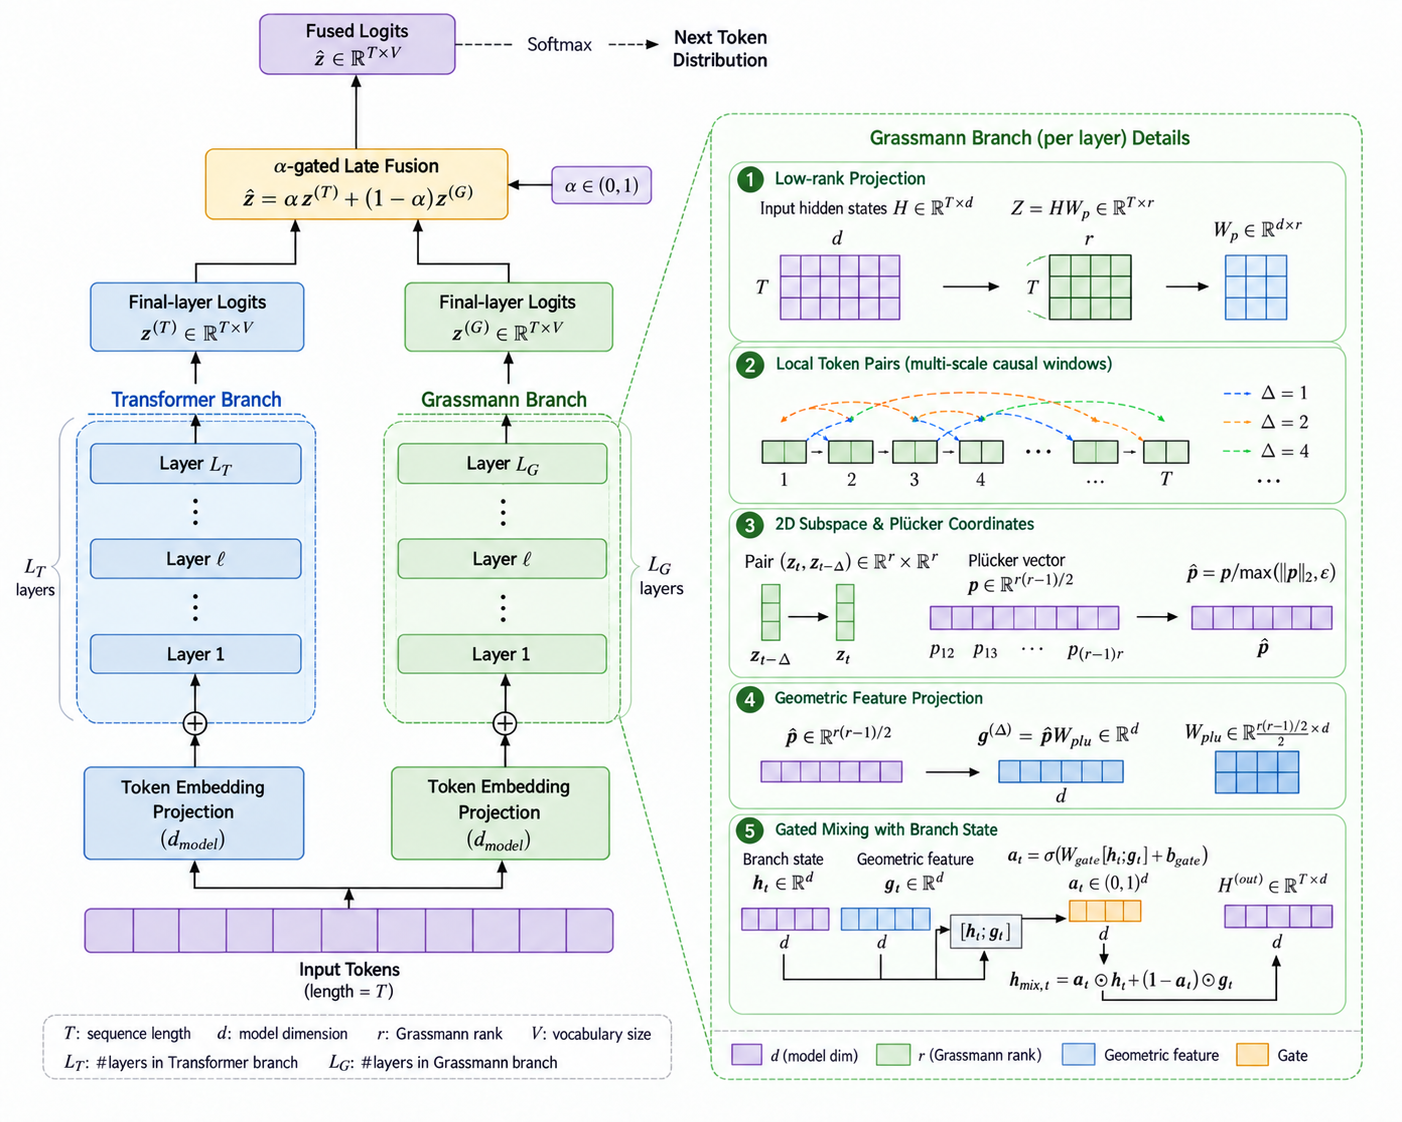
\includegraphics[width=0.94\textwidth]{figures/image1_1.png}
\caption{Shared late-fusion architecture of the teacher and hybrid students.
The Transformer and Grassmann branches independently produce final-layer
logits, which are combined by the learned scalar gate $\alpha$.  The inset
expands the Grassmann mixing operation: causal multi-scale token pairs are
encoded by normalized Pl\"ucker coordinates, projected to the model dimension,
averaged over valid offsets, and combined with the branch state through a
feature-wise gate.  The teacher and students share this topology but differ in
capacity and training.  Projection biases, residual connections, layer
normalization, dropout, and feed-forward sublayers are omitted from the
diagram.}
\label{fig:architecture}
\end{figure*}

\section{Experiments}

\subsection{Protocol and Evidence Scope}

All models use the GPT-2 tokenizer with a vocabulary of 50,257 tokens, a
sequence length of 256, a dropout rate of 0.1, and AdamW.  CE student baselines
use a learning rate of $2\times10^{-4}$.  Joint teacher training uses a
learning rate of $10^{-5}$ for the branch parameters, while KD uses
$10^{-4}$ with a cosine schedule.  The batch size is 32 for the text datasets
and 16 for code because of memory constraints.  CE baselines are trained for
20 epochs on the three text datasets and 10 epochs on code; joint teacher
training and KD each last 10 epochs.  All runs use automatic mixed precision
on NVIDIA RTX 3090 GPUs.

Table~\ref{tab:data} summarizes the training subsets recorded in the run
metadata.  The Python experiments use a 5,000-file subset of CodeParrot
\cite{codeparrot2022dataset}; they do not use the full 40,000-file local training
split.  The text datasets are PTB, WikiText-2, and TinyStories
\cite{marcus1993penn,merity2016pointer,eldan2023tinystories}.  Test perplexity
is computed by applying $\exp$ to the mean next-token CE on each fixed test
split.

\begin{table}[t]
\caption{Datasets and model sizes.  Token counts are recorded before
sequences are divided into 256-token chunks.  The code teacher and student
have equal parameter counts, so the code experiment evaluates knowledge
transfer rather than compression.}
\label{tab:data}
\centering
\footnotesize
\setlength{\tabcolsep}{3.4pt}
\begin{tabular}{lrrr}
\toprule
Dataset & Training subset & Teacher & Student \\
 &  & (M params) & (M params) \\
\midrule
PTB & 1.14M tokens & 36.26 & 31.43 \\
WikiText-2 & 2.40M tokens & 37.75 & 31.43 \\
TinyStories & 300k stories & 36.26 & 31.43 \\
Python code & 5k files & 31.43 & 31.43 \\
\bottomrule
\end{tabular}
\end{table}

Most coefficient-sweep results across the four domains are based on a single
run with seed 42.  We report descriptive differences without claims of
statistical significance.  Results from three PTB seeds are available only
for the $\lambda=0.05$ operating points discussed in
Section~\ref{sec:deployment}.  The random-initialization KD runs are not
matched to CE-from-scratch training: all use a learning rate of $10^{-4}$
rather than $2\times10^{-4}$, and the WikiText-2 and TinyStories runs use 10
rather than 20 epochs.  We therefore exclude them from the primary research
questions and discuss them only as exploratory evidence.

\subsection{RQ1: Is the Teacher More Predictive Than the Student Baseline?}

Table~\ref{tab:teachers} compares each jointly tuned fused teacher with the
CE-from-scratch hybrid student evaluated on the same dataset.  The teacher has
lower test PPL on all four datasets, although the margin is only 1.9\% on
TinyStories.  This comparison establishes that the teacher is a stronger
predictor than the student baseline; it does not isolate the contribution of
fusion because the teacher is larger on three datasets and receives additional
joint training after branch pretraining.

\begin{table}[t]
\caption{Teacher quality relative to the CE-from-scratch hybrid student (test
PPL $\downarrow$).  Negative changes indicate lower teacher PPL.}
\label{tab:teachers}
\centering
\footnotesize
\setlength{\tabcolsep}{4.2pt}
\begin{tabular}{lrrr}
\toprule
Dataset & CE student & Teacher & Relative change \\
\midrule
PTB & 58.53 & \best{50.11} & $-14.4\%$ \\
WikiText-2 & 70.16 & \best{66.87} & $-4.7\%$ \\
TinyStories & 5.07 & \best{4.97} & $-1.9\%$ \\
Python code & 7.67 & \best{5.68} & $-25.9\%$ \\
\bottomrule
\end{tabular}
\end{table}

\subsection{RQ2: Does Warm-Start KD Help Across Domains?}

For each dataset, the $\lambda=0$ run continues CE training from the same
checkpoint as the runs with positive KD coefficients, providing a matched
baseline for the effect of KD.  Table~\ref{tab:warmstart} and
Fig.~\ref{fig:sweep} show that this effect varies by domain.  The best tested
positive coefficient reduces PPL relative to CE continuation by 13.2\% on
PTB, 15.0\% on WikiText-2, and 17.2\% on code.  On TinyStories, the lowest
PPL occurs at $\lambda=0$; even the best tested positive coefficient
increases PPL by 9.3\%.

\begin{table*}[t]
\caption{Warm-start results (test PPL $\downarrow$).  ``Best WS+KD'' reports
the lowest PPL among $\lambda\in\{0.01,0.02,0.03,0.04\}$.
$\Delta$ denotes the percentage change relative to matched WS+CE; negative
values indicate improvement from KD.}
\label{tab:warmstart}
\centering
\small
\setlength{\tabcolsep}{7pt}
\begin{tabular}{lrrrrr}
\toprule
Dataset & CE scratch & WS+CE ($\lambda=0$) & Best WS+KD ($\lambda$) & Teacher & $\Delta$ vs. WS+CE \\
\midrule
PTB & 58.53 & 59.08 & \best{51.27} (0.02) & 50.11 & \best{$-13.2\%$} \\
WikiText-2 & 70.16 & 71.57 & \best{60.83} (0.02) & 66.87 & \best{$-15.0\%$} \\
TinyStories & 5.07 & \best{4.86} & 5.31 (0.01) & 4.97 & $+9.3\%$ \\
Python code & 7.67 & 7.25 & \best{6.00} (0.01) & 5.68 & \best{$-17.2\%$} \\
\bottomrule
\end{tabular}
\end{table*}

\begin{figure*}[t]
\centering
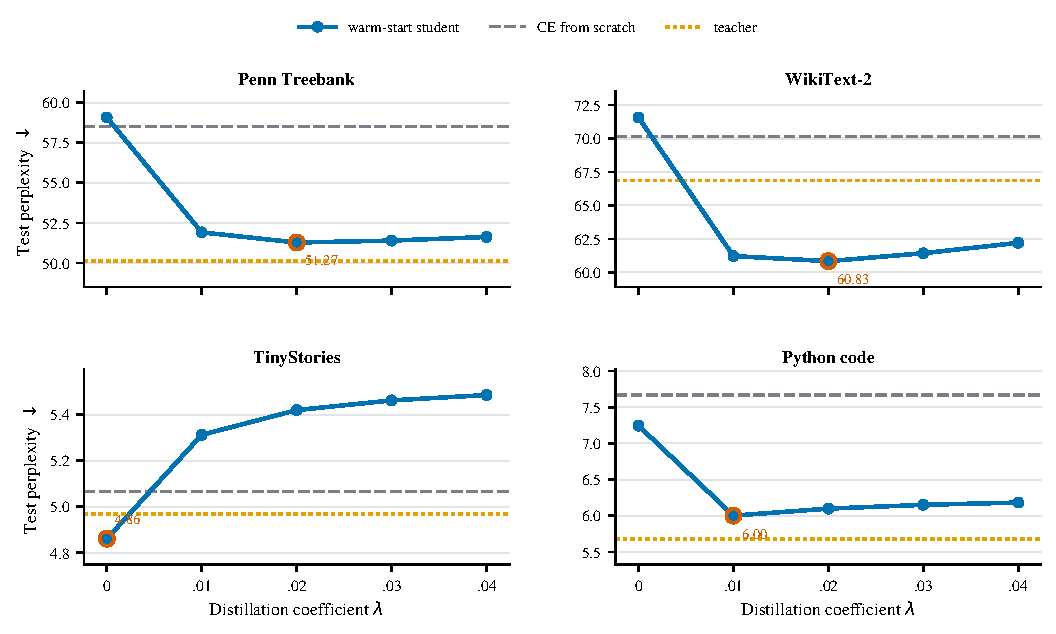
\includegraphics[width=0.98\textwidth]{figures/fig_lambda_sweep.pdf}
\caption{Warm-start coefficient sweeps.  Each panel uses a separate PPL
scale.  Gray dashed and orange dotted lines indicate the CE-from-scratch
baseline and teacher, respectively.  The circled point marks the lowest
tested PPL, including $\lambda=0$.  The lowest values occur at
$\lambda=0.02$ for PTB and WikiText-2 and at 0.01 for code.  On TinyStories,
every positive coefficient increases PPL.  Each point represents a single run.}
\label{fig:sweep}
\end{figure*}

The PPL gap between the teacher and the CE-from-scratch baseline alone does
not explain this pattern.  On TinyStories, the teacher achieves lower PPL
than the baseline (4.97 versus 5.07), yet KD increases PPL for the warm-start
student.  On WikiText-2, the student achieves 60.83 PPL, below the teacher
value of 66.87.  This result is consistent with the combined objective: the
student learns from ground-truth CE supervision as well as teacher
predictions and is not constrained to reproduce the teacher distribution.

\subsection{RQ3: What PTB Quality--Efficiency Trade-off Is Verified?}
\label{sec:deployment}

Table~\ref{tab:deployment} reports the PTB quality--efficiency trade-off using
models measured with the same batch-size benchmark.  The evaluated students use $\lambda=0.05$;
the later single-seed sweep identifies 0.02 as the best tested coefficient.
The accuracy student has 13.3\% fewer parameters than the teacher and
achieves 51.84 PPL while reducing latency by 13.4\% at batch size 32.
The 23.57M-parameter efficiency student increases PPL by 3.76 relative to the
teacher but reduces batch-32 latency by 37.6\%.

\begin{table}[t]
\caption{PTB operating points.  End-to-end batch latency is measured at a
sequence length of 256 on a single RTX 3090.}
\label{tab:deployment}
\centering
\footnotesize
\setlength{\tabcolsep}{3.0pt}
\begin{tabular}{lrrr}
\toprule
Model & PPL $\downarrow$ & Params (M) & B32 latency (ms) \\
\midrule
Teacher & \best{50.11} & 36.26 & 55.98 \\
Accuracy student & 51.84 & 31.43 & 48.46 \\
Efficiency student & 53.87 & \best{23.57} & \best{34.96} \\
\bottomrule
\end{tabular}
\end{table}

Across three seeds, PPL is $51.83\pm0.05$ for the accuracy student and
$53.91\pm0.06$ for the efficiency student (mean $\pm$ standard deviation).
Figure~\ref{fig:latency} shows that the efficiency student has the lowest
latency at every tested batch size.  The accuracy student has slightly
higher latency than the teacher at batch sizes 1 and 8 and lower latency
only at batch size 32.  The observed latency reduction therefore does not
extend to online inference with individual requests.

\begin{figure}[t]
\centering
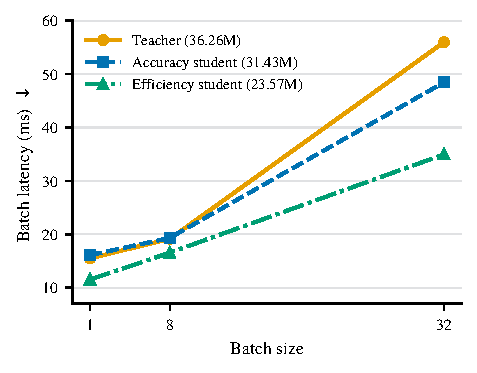
\includegraphics[width=\columnwidth]{figures/fig_batch_latency.pdf}
\caption{PTB batch-size sensitivity for the $\lambda=0.05$ operating points.
The 23.57M student has the lowest latency at all tested batch sizes; the
31.43M student has lower latency than the teacher only at batch size 32.
PPL values are 50.11 (teacher), 51.84 (accuracy student), and 53.87
(efficiency student).}
\label{fig:latency}
\end{figure}

\section{Discussion}

\subsection{Evidence and Interpretation}

The results indicate that the benefit of warm-start logit KD varies by data
domain.  After CE warm-starting, the PTB and WikiText-2
curves reach shallow minima near $\lambda=0.02$, while code achieves its
lowest PPL at 0.01 and TinyStories at zero.  The experiments do not measure
representation distance or data complexity, so an explanation based on
``geometric structure'' remains untested.

Loss normalization also affects the interpretation of the KD coefficient.
The KL term is summed over tokens and divided by batch size, whereas CE is
averaged over tokens.  At a sequence length of 256, a coefficient as small
as $\lambda=0.01$ can therefore make a substantial contribution to the
objective.  The observed preference for small coefficients applies to this
implementation and does not establish a general coefficient range for KD.

A lower teacher PPL than the CE-from-scratch baseline does not by itself
predict a benefit from KD.  KD increases PPL on TinyStories despite this
teacher advantage, whereas the WikiText-2 student trained with CE+KD
achieves lower PPL than the teacher.  Teacher quality and data domain should
therefore be evaluated separately; the present comparisons do not explain
which dataset properties determine the outcome.

\subsection{Exploratory Random-Initialization Runs}

At $\lambda=0.05$, the available random-initialization KD runs yield 123.17
PPL on WikiText-2, 5.84 on TinyStories, and 7.10 on code, compared with
CE-from-scratch values of 70.16, 5.07, and 7.67.  These comparisons do not
isolate the effect of initialization or KD because the learning rates differ,
and the two text-dataset comparisons also use different training lengths.
They suggest that a matched random-initialization study is worthwhile, but
they do not establish whether warm-starting is necessary.  We also exclude an
available PTB run with 105.86 PPL because it uses a smaller $d=192$ student and
$\lambda=0.30$.

\subsection{Cross-Domain Stress Test}

Exploratory PTB$\rightarrow$code runs yield 4.17 PPL for CE fine-tuning
initialized from a PTB student, 9.10 for KD with a PTB teacher, and 18.30 for
joint tuning of PTB branches on code.  These results are excluded from the
main comparisons because the runs use 40,000 code training files, whereas
the same-domain code experiments in Tables~\ref{tab:teachers} and
\ref{tab:warmstart}
use 5,000.  The 4.17 PPL result therefore reflects both a different source
initialization and an eightfold increase in the number of target-domain
training files.  Evaluations with matched data budgets are required to
isolate the benefit of cross-domain initialization.

\section{Limitations}

The coefficient sweeps and cross-domain comparisons use a single seed;
three-seed estimates are available only for the PTB $\lambda=0.05$
deployment points.  The models contain 23.57M--37.75M parameters, and the code
teacher has the same parameter count as the student.  The evidence therefore
supports conclusions about knowledge transfer and modest compression on
PTB, with limited applicability to large-scale model compression.  The four
datasets also differ in both domain and data volume, preventing attribution
of KD outcomes to a specific dataset property.  Batch-mean KL
normalization makes the reported coefficients implementation-specific.  The
available random-initialization and CE-from-scratch runs do not match in
learning rate, and the text-dataset runs also differ in training length, so
they cannot support a causal conclusion about initialization.
Teacher construction includes additional joint training, and the available
hidden-fusion run uses different source checkpoints from the late-fusion run.
These differences limit conclusions about the effect of fusion alone.

% TODO: additional experiment recommended: repeat lambda={0,0.01,0.02,0.03}
% with at least three seeds on every dataset and report confidence intervals.
% TODO: additional experiment recommended: compare batch-mean and token-mean
% KL normalization and retune lambda under both definitions.
% TODO: additional experiment recommended: rerun PTB late/hidden fusion from
% identical branch checkpoints and equalize parameter counts/training steps.
% TODO: additional experiment recommended: rerun PTB->code transfer with the
% same 5k or 40k target-domain files for every baseline and teacher route.

\section{Conclusion}

We examined how warm-start logit KD from a heterogeneous
Grassmann--Transformer teacher behaves across text domains.  After CE
warm-starting, KD
reduces perplexity on PTB, WikiText-2, and Python code, but increases it on
TinyStories.  The available random-initialization runs are not matched to the
CE baselines and therefore do not establish an initialization effect.  These
results support tuning and replicating KD coefficients separately for each
domain.  On PTB, warm-start KD yields two practical operating points: a
31.43M student achieves perplexity close to that of the teacher with lower
large-batch latency, while a 23.57M student provides a larger latency
reduction at the cost of higher perplexity.  Further evaluation should use
multiple seeds, token-normalized losses, and matched fusion and cross-domain
controls to test how well these findings extend beyond the current settings.

\bibliographystyle{IEEEtran}
\bibliography{refs}

\end{document}
